\chapter*{Melakukan Login Otomatis}

\begin{enumerate}
	\item Mengetikan scrip seperti di gambar 
	\begin{figure} [h]
	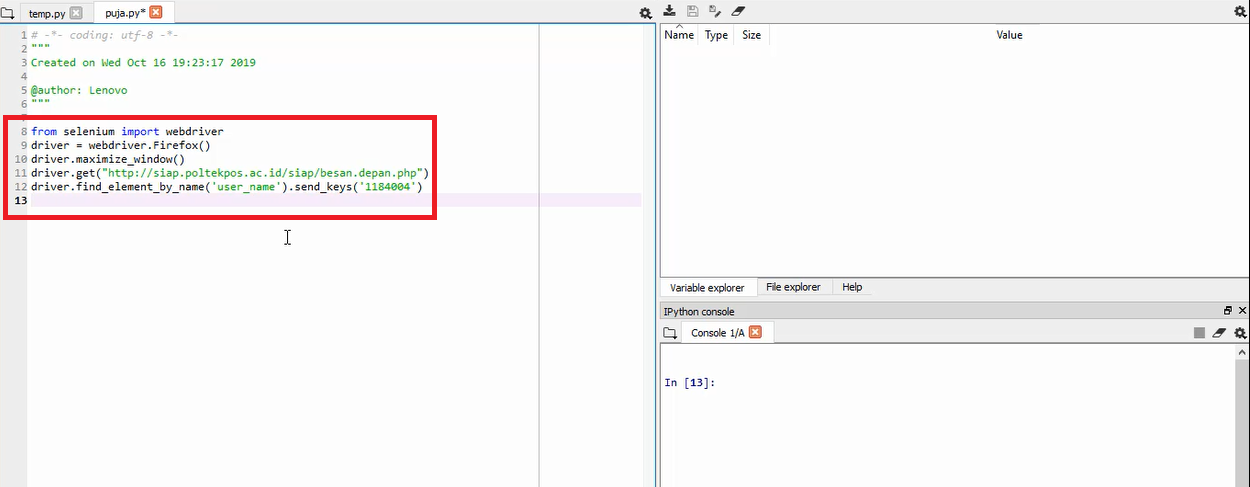
\includegraphics[width=5cm]{login/1.png}
	\centering
	\end{figure}
	
	\item Meng-copy kan link SIAP dan masukan kodingan username dan pasword sesuai akun yang kita miliki
	\begin{figure} [h]
	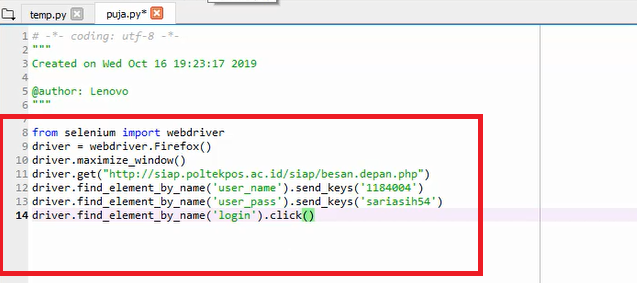
\includegraphics[width=5cm]{login/2.png}
	\centering
	\end{figure}

	\item Masuk ke web siap lalu arahkan krusor ke bagian login dan klik kanan inspect elements 
	\begin{figure} [h]
	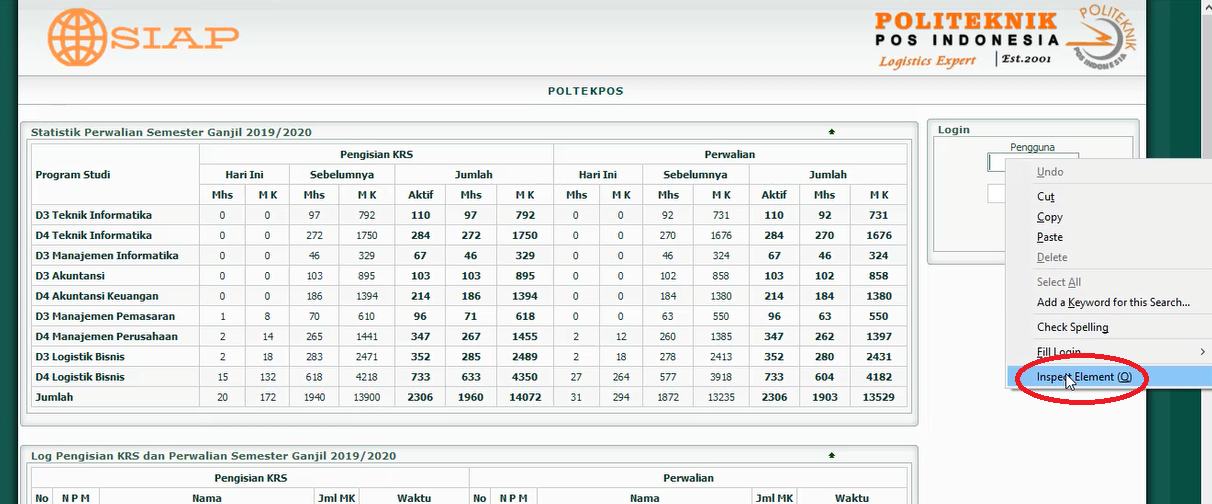
\includegraphics[width=5cm]{login/3.png}
	\centering
	\end{figure}
	
	\item Sampai keluar seperti digambar
	\begin{figure} [h]
	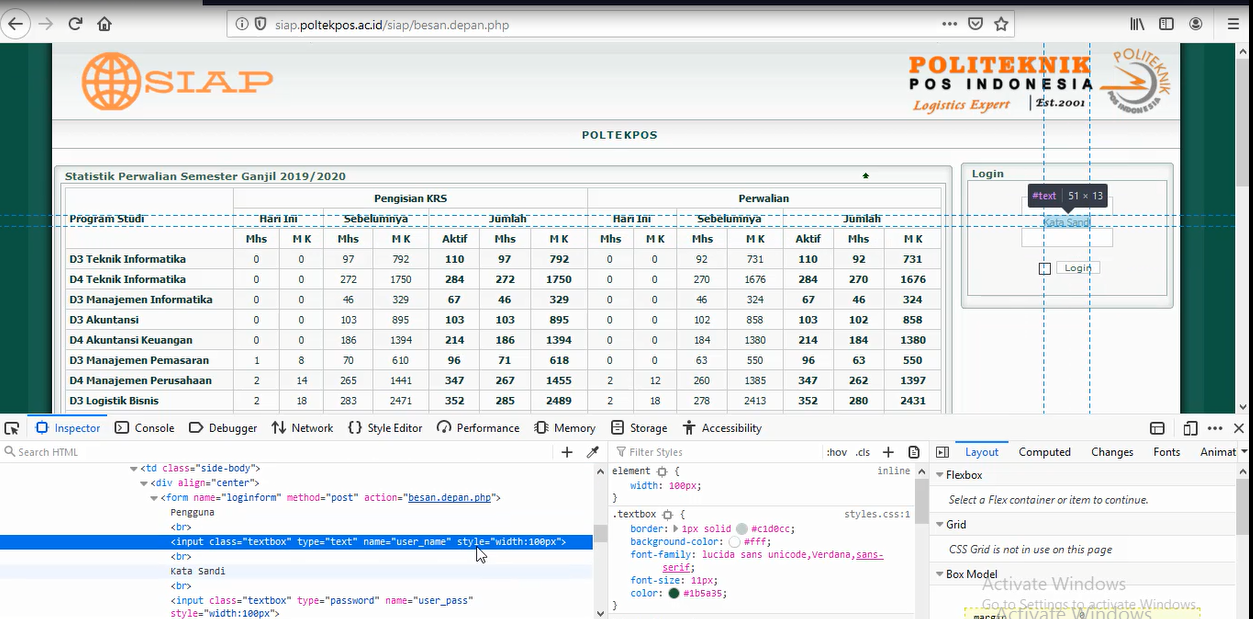
\includegraphics[width=5cm]{login/4.png}
	\centering
	\end{figure}
	
	\item Lalu masukan username dan pasword kita
	\begin{figure} [h]
	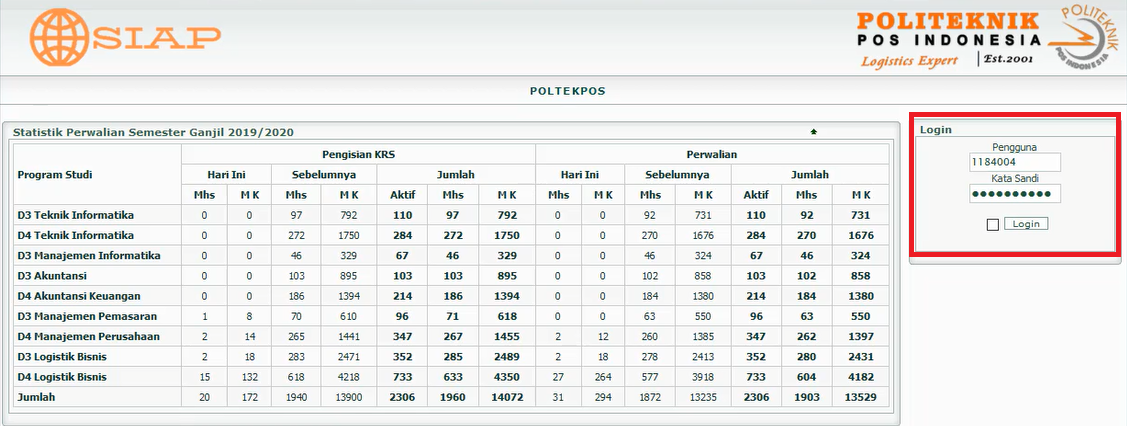
\includegraphics[width=6cm]{login/5.png}
	\centering
	\end{figure}
	
	\item Lalu loading login seperti di gambar 
	\begin{figure} [h]
	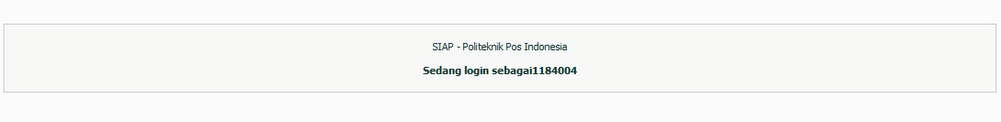
\includegraphics[width=6cm]{login/6.png}
	\centering
	\end{figure}
	
	\item Dan sudah terlogin seperti digambar 
	\begin{figure} [h]
	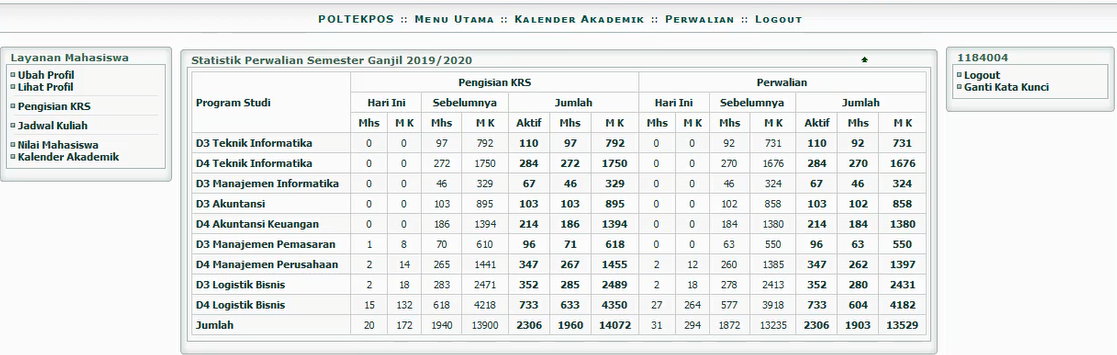
\includegraphics[width=6cm]{login/7.png}
	\centering
	\end{figure}
	

\end{enumerate}
